\chapter{Vurdering af vores løsning}
\label{Evaluation}
\section{Opfyldelse af kravspecifikation}
\label{Evaluation_KS}
\subsection{Nuværende og ønsket situation}
\label{Evaluation_KS_situation}
Kravspecifikationen beskriver den nuværende situation som værende uoverskuelig og besværlig, fordi planlægning og booking foregår i mange forskellige systemer. Facility Management (FM) er centralt bindepunkt for alt vedrørende lokaleadministration (se figur \ref{Fig:Evaluation_KS_situation_current}). 

\begin{figure}[h!]
  \centering
    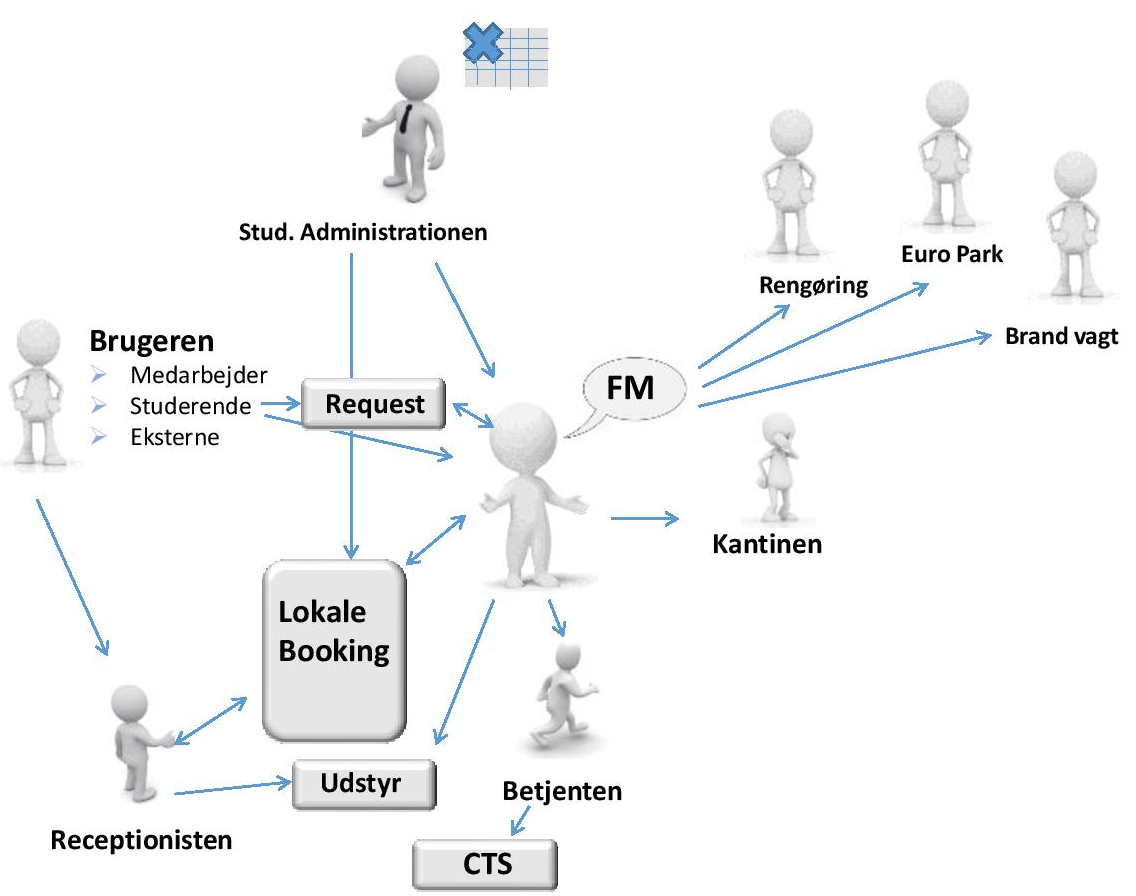
\includegraphics[width=0.75\textwidth]{Appendix/GUI-Prototype/NuvaerendeFlow}
  \caption{Flowchart af den nuværende situation\cite[s. 4]{kravspec}.}
\label{Fig:Evaluation_KS_situation_current}
\end{figure}

De forretningsmæssige mål med en integeret løsning til booking af lokalet er bl.a. at effektivisere resurseforbrug, minimere fejl og aflaste aflaste medarbejdere. I forbindelse med disse mål beskriver kravspecifikationen en vision for den ønskede løsning (se figur \ref{Fig:Evaluation_KS_situation_goal}).

\begin{figure}[h!]
  \centering
    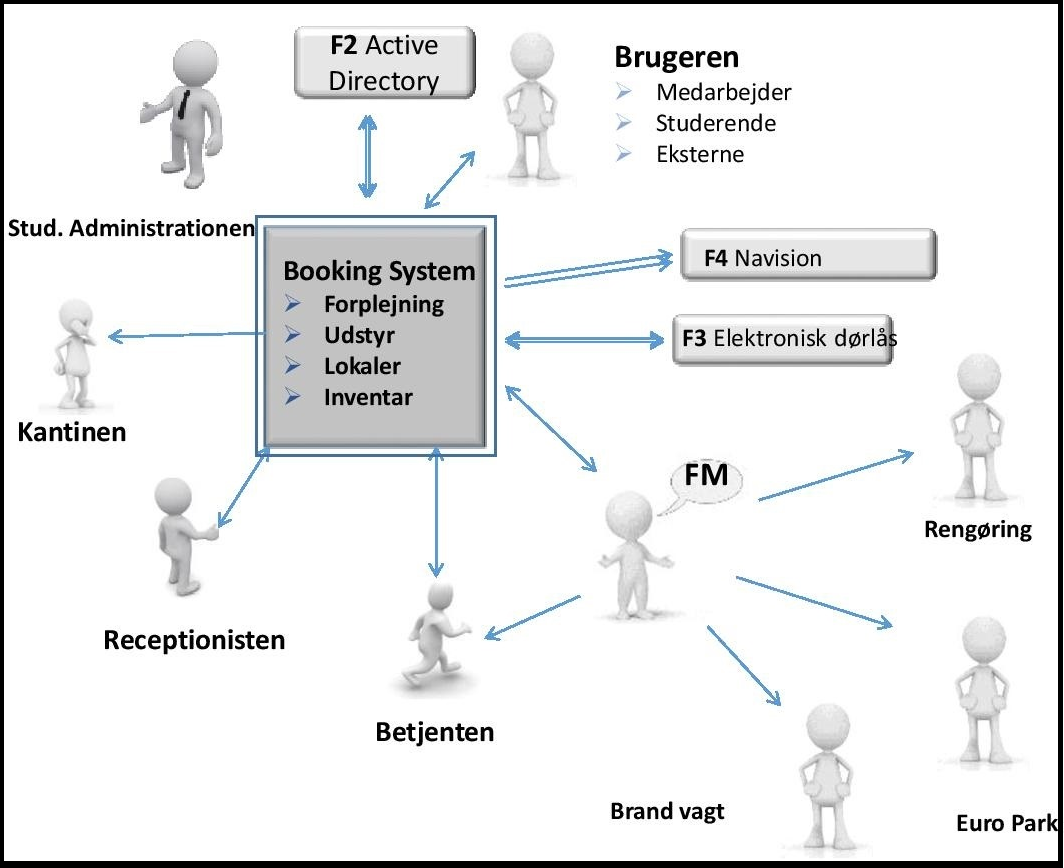
\includegraphics[width=\textwidth]{Appendix/GUI-Prototype/DesiredFlow}
  \caption{Flowchart af visionen af den ønskede løsning\cite[s. 4]{kravspec}.}
\label{Fig:Evaluation_KS_situation_goal}
\end{figure}

Vi mener, at vores løsning et tæt på denne vision, hvis løsningen bliver fuldt implementeret. Skærmbillederne i vores løsning understøtter mange af de elementer, som visionen består af. De vigtigste elementer, vi ikke understøtter, er redigeringsmuligheder til forplejningselementer og eksterne brugere\footnote{Skærmbillederne udelukker ikke helt, at eksterne brugere kan anvende systemet. Priser på lokaler og udstyr er dog en del af de eksterne brugeres anvendelse af systemer, hvilket vores skærmbilleder ikke understøtter.}.

\subsection{Understøttede arbejdsopgaver}
\label{Evaluation_KS_workareas}
Kravspecifikationen definerer 13 arbejdsopgaver:
\begin{my_description}
\item[\textbf{C1.}]{Administrer booking}
\item[\textbf{C2.}]{Forespørg på booking}
\item[\textbf{C3.}]{Modtag forespørgsel fra Ekstern}
\item[\textbf{C4.}]{Klargør lokaler}
\item[\textbf{C5.}]{Udlevér nøgle}
\item[\textbf{C6.}]{Håndtér forplejning}
\item[\textbf{C7.}]{Fakturér forplejning}
\item[\textbf{C8.}]{Opdatér menukort}
\item[\textbf{C9.}]{Opdater listen for ekstra udstyr}
\item[\textbf{C10.}]{Opdatér lokaler}
\item[\textbf{C11.}]{Administrér bruger}
\item[\textbf{C12.}]{Håndter statistik}
\item[\textbf{C13.}]{Behandl faktura}
\end{my_description}

Ud af de 13 arbejdesopgaver understøtter vi \textbf{C1}, \textbf{C9} og \textbf{C10}. Hver af arbejdsopgaverne har en række underpunkter, som beskriver delopgaver og varianter af disse delopgaver. 
\\Vi har indsat den overordnede beskrivelse af arbejdsopgaverne samt tabellerne over delopgaver/varianter. Vi har tilføjet to kolonner til tabellerne: "Understøttet" og "Vores Løsning". "Vores Løsning" beskriver, hvilket skærmbillede løser delopgaven.

\subsubsection{C1: Administrer booking}
\textbf{Brugere:} Ansatte og studerende på ITU.\\
\textbf{Hyppighed:} Flere gange om dagen i alt for både studerende og ansatte.\\
\textbf{Start:} En person går ind i booking systemet for at booke, ændre eller få overblik over bookinger.\\
\textbf{Slut:} Når bookingen eller ændringen er foretaget.

\begin{tabular}{ | p{7.5cm} | p{2.5cm} | p{2.2cm} | p{3.3cm} |}
\hline
\textbf{Arbejdesopgave} & \textbf{Eks. løsning} & \textbf{Understøttet}  & \textbf{Vores løsning}\\ 
\hline
1. Søg efter ledigt tidspunkt for ny booking & & Ja & Billede \ref{App_GUI_final_GridEksempel}(side \pageref{App_GUI_final_GridEksempel}) \\ 
\hline
1a. Søg efter eksisterende booking &  & Ja & Billede \ref{App_GUI_final_DineBookinger}(side \pageref{App_GUI_final_DineBookinger}) \\ 
\hline
2. Vælg ledigt lokale, forplejning og ekstra udstyr & & Ja & \begin{tabular}[t]{@{}l@{}}Billede \ref{App_GUI_final_DineBookinger}(side \pageref{App_GUI_final_DineBookinger})\&\\Billede \ref{App_GUI_final_Forplejning}(side \pageref{App_GUI_final_Forplejning})\&\\Billede \ref{App_GUI_final_BookEquip}(side \pageref{App_GUI_final_BookEquip})    \end{tabular}\\
\hline
2a. Vis eksisterende booking(er) & & Ja & Billede \ref{App_GUI_final_GridEksempel}(side \pageref{App_GUI_final_GridEksempel})\\ 
\hline
3. Opdater booking & & Ja & Billede \ref{App_GUI_final_GridEksempel}(side \pageref{App_GUI_final_GridEksempel})\\ 
\hline
4. Annuller booking & & Ja & Billede \ref{App_GUI_final_DineBookinger}(side \pageref{App_GUI_final_DineBookinger})\\ 
\hline
5. Opret booking & & Ja & Billede \ref{App_GUI_final_GridEksempel}(side \pageref{App_GUI_final_GridEksempel})\\ 
\hline
\end{tabular}

\subsubsection{C9: Opdater listen for ekstra udstyr}
\textbf{Brugere:} Facility Management (FM)\\
\textbf{Hyppighed:} Når der sker ændring i udvalget af ekstra udstyr (en gang om måneden)\\
\textbf{Start:} Når der er behov for at udstyrslisten skal opdateres\\
\textbf{Slut:} Når listen er opdateret

\begin{tabular}{ | p{7.5cm} | p{2.5cm} | p{2.2cm} | p{3.3cm} |}
\hline
\textbf{Arbejdesopgave} & \textbf{Eks. løsning} & \textbf{Understøttet}  & \textbf{Vores løsning}\\ 
\hline
C9.1 Rediger udstyrslisten & FM er ansvarlig & Ja & Billede \ref{App_GUI_final_UdstyrsListe}(side \pageref{App_GUI_final_UdstyrsListe}) \\ 
\hline
\end{tabular}

\subsubsection{C10: Opdatér lokaler}
\textbf{Brugere:} Facility Management (FM)\\
\textbf{Hyppighed:} Når der sker ændring i antallet af lokaler til bookingen (en gang om måneden)\\
\textbf{Start:} Når der er behov for at lokalelisten skal opdateres\\
\textbf{Slut:} Når listen er opdateret

\begin{tabular}{ | p{7.5cm} | p{2.5cm} | p{2.2cm} | p{3.3cm} |}
\hline
\textbf{Arbejdesopgave} & \textbf{Eks. løsning} & \textbf{Understøttet}  & \textbf{Vores løsning}\\ 
\hline
C10.1 Rediger lokalelisten & & Ja & Billede \ref{App_GUI_final_LokaleListe}(side \pageref{App_GUI_final_LokaleListe}) \\ 
\hline
C10.2 Rediger lokale inventar & & Ja & Billede \ref{App_GUI_final_AendreLokale}(side \pageref{App_GUI_final_AendreLokale}) \\ 
\hline
\end{tabular}

\subsubsection{Prioritering af arbejdsopgaver}
\label{Evaluation_workareas_priorities}
I denne første release har vi valgt at fokusere på at understøtte booking af lokaler, udstyr og forplejning for interne brugere på IT-Universitetet. De arbejdsopgaver, vi understøtter, er derfor dem, som gør dette muligt.

Vi mener, det er en kernefunktionalitet i systemet, hvilket gør det vigtigt at understøtte i tidlige udgaver af systemet. \\Kravspecifikationen vægter arbejdsopgave \textbf{C1} \& \textbf{C2} som en $\frac{1}{5}$ af den fulde vægt, hvilket betyder, at dette punkt betyder meget for kunden\cite[s. 8]{kravspec}.

Da en stor del af vægtningen i minimumskravene er \textbf{C1}-\textbf{C5} (samlet $\frac{2}{5}$ af vægtningen), vil vi foreslå, at man prioriterer \textbf{C2}, \textbf{C3}, \textbf{C4} og \textbf{C5} i forbindelse med videreudvikling af systemet.
\\Derudover har \textbf{C13} en vægtning på $\frac{1}{10}$.  Man kunne derfor overveje at prioritere \textbf{C13} højere end enkelte delopgaver/variationer af \textbf{C2}-\textbf{C5}. Dette bør dog komme an på en vurdering af omkostningen af \textbf{C13} kontra udvidet funktionalitet i forbindelse med andre arbejsopgaver.

\section{Future release}
\label{Evaluation_Future}
\subsection{Request for change}
\label{Evaluation_Future_RFC}
Det er nødvendigt med en ændring i Active Directory, hvis det skal understøtte flere roller i forbindelse med booking systemet. 
\\En mulig løsning er at lave en attribut "ituRoles" med format "Role1;Role2;...", fx "ituRoles='Cantine;Student;'". 
\\En anden løsning kunne være at udvide/ændre "ituAffiliation" til at anvende samme format.

\subsection{"Future Release"-liste}
\label{Evaluation_Future_FR}
Elementerne på vores "future release"-liste bør diskuteres med kunden før udvikling. Hvert element bør vurderes i forhold til både nytteværdi og omkostning for kunden. 
\\Dette kunne eventuelt gøres ved, at kunden giver en vurdering af nytteværdien og udvikleren giver en vurdering af omkostningen. Disse værdier kunne så bruges til at lave en cost/benefit-analyse, som ville vise, hvilke elementer bør prioriteres højest.

Vores "future release"-liste består af følgende elementer (ikke prioriteret rækkefølge):
\begin{my_description}
\item[Fejlrettelse] Rettelse af defekter og "Not Yet Implemented" fundet under test.
\item[Nye arbejdsopgaver] Understøttelse af flere arbejdsopgaver (som skrevet i afsnit \ref{Evaluation_workareas_priorities})
\item[Forbedret teststrategi] Indfasning af en forbedret teststrategi (beskrevet i afsnit \ref{Test_intendedStrat})
\item[Usability Test] Usability test (og håndtering af eventuelle usability problemer)
\item[Nye platforme] Udvikling af klient til fx mobiltelefoner.
\item[Brugergrænseflade] Ændringer til brugergrænsefladen, som beskrevet i afsnit \ref{Evaluation_Future_GUI}.
\end{my_description}

\subsection{Ændringer til brugergrænsefladen}
\label{Evaluation_Future_GUI}
\subsubsection{Ydeligere understøttelse af arbejdsopgaver}
Følgende er en liste over ændringer, vi mener skal foretages, for at systemet understøtter en større del af arbejdsopgaverne:
\begin{my_itemize}
\item Understøt godkendelse af forplejning og udstyrsvalg
\item Tilføjelse af nye typer forplejning og nye udstyrstyper
\item Mulighed for at ændre indhold af forplejningsliste
\item Mulighed for at angive antal deltagere til en booking
\item Mulighed for at administrator kan ændre bookinger
\end{my_itemize}

\subsubsection{Usability ændringer}
Følgende er en liste af ændringer, som vi mener gøre systemet nemmere at anvende:
\begin{my_itemize}
\item Brugerens egne bookinger skal være øverst på listen over bookinger
\item Sammenlægning af "Booking-Liste" og "Find Bookinger"
\item Sammenlægning af "Konfigurering af Lokaler" og "Ændre Lokale"
\item Informering om ændringer i status på en brugers booking
\item Mulighed for at skifte mellem sprog (dansk/engelsk)
\item Være i stand til at søge på sal i lokalelisten
\item Paging på alle sider med gittrer
\end{my_itemize}
